\begin{figure}[tbp]
\centering
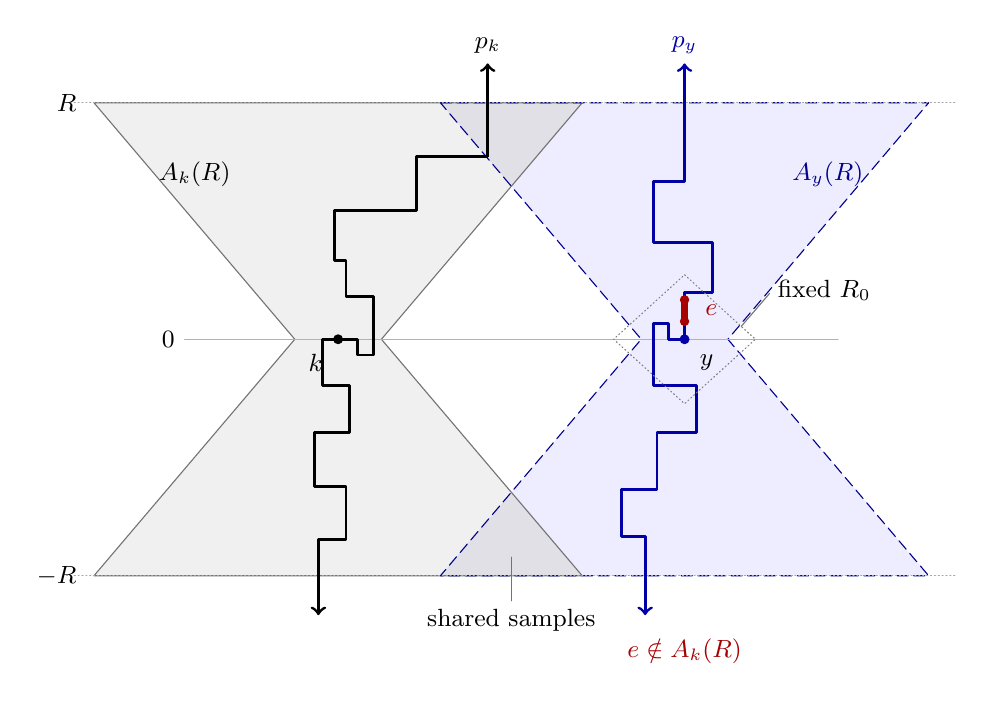
\begin{tikzpicture}[x=1cm,y=.91cm,font=\small,
  line cap=round,line join=round]
  \fill[black!6] (-5.3,3.3)--(.9,3.3)--(-1.65,0)
    --(.9,-3.3)--(-5.3,-3.3)--(-2.75,0)--cycle;
  \fill[blue!7!white] (-.9,3.3)--(5.3,3.3)--(2.75,0)
    --(5.3,-3.3)--(-.9,-3.3)--(1.65,0)--cycle;
  \fill[blue!18!black!12] (0,2.1353)--(.9,3.3)--(-.9,3.3)--cycle;
  \fill[blue!18!black!12] (0,-2.1353)--(.9,-3.3)--(-.9,-3.3)--cycle;
  \draw[black!55] (-5.3,3.3)--(.9,3.3)--(-1.65,0)
    --(.9,-3.3)--(-5.3,-3.3)--(-2.75,0)--cycle;
  \draw[blue!55!black,dash pattern=on 4pt off 2pt]
    (-.9,3.3)--(5.3,3.3)--(2.75,0)
    --(5.3,-3.3)--(-.9,-3.3)--(1.65,0)--cycle;
  \draw[black!35,densely dotted] (-5.65,3.3)--(5.65,3.3);
  \draw[black!35,densely dotted] (-5.65,-3.3)--(5.65,-3.3);
  \draw[black!30] (-4.15,0)--(4.15,0);
  \node[left] at (-5.4,3.3) {$R$};
  \node[left] at (-5.4,-3.3) {$-R$};
  \node[left] at (-4.15,0) {$0$};
  \node at (-4.02,2.3) {$A_k(R)$};
  \node[text=blue!55!black] at (4.02,2.3) {$A_y(R)$};

  \draw[line width=1.05pt,->]
    (-2.2,0)--(-1.95,0)--(-1.95,-.22)--(-1.75,-.22)
    --(-1.75,.6)--(-2.1,.6)--(-2.1,1.1)--(-2.25,1.1)
    --(-2.25,1.8)--(-1.2,1.8)--(-1.2,2.55)--(-.3,2.55)
    --(-.3,3.85);
  \draw[line width=1.05pt,->]
    (-2.2,0)--(-2.4,0)--(-2.4,-.65)--(-2.05,-.65)
    --(-2.05,-1.3)--(-2.5,-1.3)--(-2.5,-2.05)
    --(-2.1,-2.05)--(-2.1,-2.8)--(-2.45,-2.8)--(-2.45,-3.85);
  \draw[blue!65!black,line width=1.05pt,->]
    (2.2,0)--(2.2,.65)--(2.55,.65)--(2.55,1.35)
    --(1.8,1.35)--(1.8,2.2)--(2.2,2.2)--(2.2,3.85);
  \draw[blue!65!black,line width=1.05pt,->]
    (2.2,0)--(2,0)--(2,.22)--(1.8,.22)--(1.8,-.65)
    --(2.35,-.65)--(2.35,-1.3)--(1.85,-1.3)
    --(1.85,-2.1)--(1.4,-2.1)--(1.4,-2.75)
    --(1.7,-2.75)--(1.7,-3.85);
  \node[above] at (-.3,3.85) {$p_k$};
  \node[above,text=blue!65!black] at (2.2,3.85) {$p_y$};
  \fill (-2.2,0) circle (1.8pt);
  \fill[blue!65!black] (2.2,0) circle (1.8pt);
  \node[below left=2pt] at (-2.2,0) {$k$};
  \node[below right=2pt] at (2.2,0) {$y$};

  \draw[black!50,densely dotted] (2.2,.9)--(3.1,0)
    --(2.2,-.9)--(1.3,0)--cycle;
  \draw[red!65!black,line width=2.5pt] (2.2,.25)--(2.2,.55);
  \fill[red!65!black] (2.2,.25) circle (1.7pt)
    (2.2,.55) circle (1.7pt);
  \node[right=4pt,text=red!65!black] at (2.2,.4) {$e$};
  \draw[black!55] (3.28,.64)--(2.92,.18);
  \node[anchor=west] at (3.26,.68) {fixed $R_0$};
  \draw[black!55] (0,-3.65)--(0,-3.04);
  \node at (0,-3.92) {shared samples};
  \node[text=red!65!black] at (2.2,-4.35) {$e\notin A_k(R)$};
\end{tikzpicture}
\caption{Schematic envelopes of the truncated edge regions $A_k(R)$
and $A_y(R)$, not their exact lattice footprints. Overlap uses the same
raised sample for each edge, with no repeated increase. Every marked-path
edge in the slab belongs to its own region, so the union preserves both
paths' weights and geodesic property. The strictly raised edge $e$ lies
among the first $R_0$ steps from $y$ and outside $A_k(R)$ at sufficiently
large fixed separation. The near radius $R_0$ and this separation remain
fixed as $R$ grows.}
\label{fig:union}
\end{figure}
